\documentclass[12pt]{report}
\usepackage{scribe,graphicx,graphics}
\usepackage{proba}
\usepackage{float}
\usepackage{cancel}
\usepackage{listings}
\newcommand{\norm}[1]{\left|\left|#1\right|\right|}
\usepackage{listings}
\usepackage{xcolor}
\usepackage{listings}
\DeclareMathOperator*{\Tr}{Tr}
\definecolor{codegreen}{rgb}{0,0.6,0}
\definecolor{codegray}{rgb}{0.5,0.5,0.5}
\definecolor{codepurple}{rgb}{0.58,0,0.82}
\definecolor{backcolour}{rgb}{0.95,0.95,0.92}

\lstdefinestyle{mystyle}{
    backgroundcolor=\color{backcolour},   
    commentstyle=\color{codegreen},
    keywordstyle=\color{magenta},
    numberstyle=\tiny\color{codegray},
    stringstyle=\color{codepurple},
    basicstyle=\ttfamily\footnotesize,
    breakatwhitespace=false,         
    breaklines=true,                 
    captionpos=b,                    
    keepspaces=true,                 
    numbers=left,                    
    numbersep=5pt,                  
    showspaces=false,                
    showstringspaces=false,
    showtabs=false,                  
    tabsize=2
}

\lstset{style=mystyle}
\course{CSE 382M} 	
\coursetitle{Found. Data Science \& ML}	
\semester{Spring 2025}
\lecturer{} % Due Date: {\bf Mon, Oct 3 2016}}
\lecturetitle{Problem Set}
\lecturenumber{3}   
\lecturedate{}    
\usepackage{enumerate}
\newcommand{\remind}[1]{\textcolor{red}{\textbf{#1}}} %To remind me of unfinished work to fix later
\newcommand{\hide}[1]{} %To hide large blocks of code without using % symbols

\newcommand{\ep}{\varepsilon}
\newcommand{\vp}{\varphi}
\newcommand{\lam}{\lambda}
\newcommand{\Lam}{\Lambda}
%\newcommand{\abs}[1]{\ensuremath{\left\lvert#1\right\rvert}} % This clashes with the physics package
%\newcommand{\norm}[1]{\ensuremath{\left\lVert#1\right\rVert}} % This clashes with the physics package
\newcommand{\floor}[1]{\ensuremath{\left\lfloor#1\right\rfloor}}
\newcommand{\ceil}[1]{\ensuremath{\left\lceil#1\right\rceil}}
\newcommand{\A}{\mathbb{A}}
\newcommand{\B}{\mathbb{B}}
\newcommand{\C}{\mathbb{C}}
\newcommand{\D}{\mathbb{D}}
\newcommand{\E}{\mathbb{E}}
\newcommand{\F}{\mathbb{F}}
\newcommand{\K}{\mathbb{K}}
\newcommand{\N}{\mathbb{N}}
\newcommand{\Q}{\mathbb{Q}}
\newcommand{\R}{\mathbb{R}}
\newcommand{\T}{\mathbb{T}}
\newcommand{\X}{\mathbb{X}}
\newcommand{\Y}{\mathbb{Y}}
\newcommand{\Z}{\mathbb{Z}}
\newcommand{\As}{\mathcal{A}}
\newcommand{\Bs}{\mathcal{B}}
\newcommand{\Cs}{\mathcal{C}}
\newcommand{\Ds}{\mathcal{D}}
\newcommand{\Es}{\mathcal{E}}
\newcommand{\Fs}{\mathcal{F}}
\newcommand{\Gs}{\mathcal{G}}
\newcommand{\Hs}{\mathcal{H}}
\newcommand{\Is}{\mathcal{I}}
\newcommand{\Js}{\mathcal{J}}
\newcommand{\Ks}{\mathcal{K}}
\newcommand{\Ls}{\mathcal{L}}
\newcommand{\Ms}{\mathcal{M}}
\newcommand{\Ns}{\mathcal{N}}
\newcommand{\Os}{\mathcal{O}}
\newcommand{\Ps}{\mathcal{P}}
\newcommand{\Qs}{\mathcal{Q}}
\newcommand{\Rs}{\mathcal{R}}
\newcommand{\Ss}{\mathcal{S}}
\newcommand{\Ts}{\mathcal{T}}
\newcommand{\Us}{\mathcal{U}}
\newcommand{\Vs}{\mathcal{V}}
\newcommand{\Ws}{\mathcal{W}}
\newcommand{\Xs}{\mathcal{X}}
\newcommand{\Ys}{\mathcal{Y}}
\newcommand{\Zs}{\mathcal{Z}}
\newcommand{\ab}{\textbf{a}}
\newcommand{\bb}{\textbf{b}}
\newcommand{\cb}{\textbf{c}}
\newcommand{\db}{\textbf{d}}
\newcommand{\ub}{\textbf{u}}
\newcommand{\sbb}{\textbf{s}}
%\renewcommand{\vb}{\textbf{v}} % This clashes with the physics package (the physics package already defines the \vb command)
\newcommand{\wb}{\textbf{w}}
\newcommand{\xb}{\textbf{x}}
\newcommand{\yb}{\textbf{y}}
\newcommand{\zb}{\textbf{z}}
\newcommand{\vbb}{\textbf{v}}
\newcommand{\Ab}{\textbf{A}}
\newcommand{\Bb}{\textbf{B}}
\newcommand{\Cb}{\textbf{C}}
\newcommand{\Db}{\textbf{D}}
\newcommand{\eb}{\textbf{e}}
\newcommand{\ex}{\textbf{e}_x}
\newcommand{\ey}{\textbf{e}_y}
\newcommand{\ez}{\textbf{e}_z}
\newcommand{\zerob}{\mathbf{0}}
\newcommand{\abar}{\overline{a}}
\newcommand{\bbar}{\overline{b}}
\newcommand{\cbar}{\overline{c}}
\newcommand{\dbar}{\overline{d}}
\newcommand{\ubar}{\overline{u}}
\newcommand{\vbar}{\overline{v}}
\newcommand{\wbar}{\overline{w}}
\newcommand{\xbar}{\overline{x}}
\newcommand{\ybar}{\overline{y}}
\newcommand{\zbar}{\overline{z}}
\newcommand{\Abar}{\overline{A}}
\newcommand{\Bbar}{\overline{B}}
\newcommand{\Cbar}{\overline{C}}
\newcommand{\Dbar}{\overline{D}}
\newcommand{\Ubar}{\overline{U}}
\newcommand{\Vbar}{\overline{V}}
\newcommand{\Wbar}{\overline{W}}
\newcommand{\Xbar}{\overline{X}}
\newcommand{\Ybar}{\overline{Y}}
\newcommand{\Zbar}{\overline{Z}}
\newcommand{\Aint}{A^\circ}
\newcommand{\Bint}{B^\circ}
\newcommand{\limk}{\lim_{k\to\infty}}
\newcommand{\limm}{\lim_{m\to\infty}}
\newcommand{\limn}{\lim_{n\to\infty}}
\newcommand{\limx}[1][a]{\lim_{x\to#1}}
\newcommand{\liminfm}{\liminf_{m\to\infty}}
\newcommand{\limsupm}{\limsup_{m\to\infty}}
\newcommand{\liminfn}{\liminf_{n\to\infty}}
\newcommand{\limsupn}{\limsup_{n\to\infty}}
\newcommand{\sumkn}{\sum_{k=1}^n}
\newcommand{\sumk}[1][1]{\sum_{k=#1}^\infty}
\newcommand{\summ}[1][1]{\sum_{m=#1}^\infty}
\newcommand{\sumn}[1][1]{\sum_{n=#1}^\infty}
\newcommand{\emp}{\varnothing}
\newcommand{\exc}{\backslash}
\newcommand{\sub}{\subseteq}
\newcommand{\sups}{\supseteq}
\newcommand{\capp}{\bigcap}
\newcommand{\cupp}{\bigcup}
\newcommand{\kupp}{\bigsqcup}
\newcommand{\cappkn}{\bigcap_{k=1}^n}
\newcommand{\cuppkn}{\bigcup_{k=1}^n}
\newcommand{\kuppkn}{\bigsqcup_{k=1}^n}
\newcommand{\cappk}[1][1]{\bigcap_{k=#1}^\infty}
\newcommand{\cuppk}[1][1]{\bigcup_{k=#1}^\infty}
\newcommand{\cappm}[1][1]{\bigcap_{m=#1}^\infty}
\newcommand{\cuppm}[1][1]{\bigcup_{m=#1}^\infty}
\newcommand{\cappn}[1][1]{\bigcap_{n=#1}^\infty}
\newcommand{\cuppn}[1][1]{\bigcup_{n=#1}^\infty}
\newcommand{\kuppk}[1][1]{\bigsqcup_{k=#1}^\infty}
\newcommand{\kuppm}[1][1]{\bigsqcup_{m=#1}^\infty}
\newcommand{\kuppn}[1][1]{\bigsqcup_{n=#1}^\infty}
\newcommand{\cappa}{\bigcap_{\alpha\in I}}
\newcommand{\cuppa}{\bigcup_{\alpha\in I}}
\newcommand{\kuppa}{\bigsqcup_{\alpha\in I}}
\newcommand{\Rx}{\overline{\mathbb{R}}}
\newcommand{\dx}{\,dx}
\newcommand{\dy}{\,dy}
\newcommand{\dt}{\,dt}
\newcommand{\dax}{\,d\alpha(x)}
\newcommand{\dbx}{\,d\beta(x)}
\DeclareMathOperator{\glb}{\text{glb}}
\DeclareMathOperator{\lub}{\text{lub}}
\newcommand{\xh}{\widehat{x}}
\newcommand{\yh}{\widehat{y}}
\newcommand{\zh}{\widehat{z}}
\newcommand{\<}{\langle}
\renewcommand{\>}{\rangle}
\renewcommand{\iff}{\Leftrightarrow}
\DeclareMathOperator{\im}{\text{im}}
\let\spn\relax\let\Re\relax\let\Im\relax
\DeclareMathOperator{\spn}{\text{span}}
\DeclareMathOperator{\sym}{\text{Sym}}
\DeclareMathOperator{\myskew}{\text{Skew}}
\DeclareMathOperator{\Re}{\text{Re}}
\DeclareMathOperator{\Im}{\text{Im}}
\DeclareMathOperator{\diag}{\text{diag}}
\endinput

% Insert your name here!
\scribe{Student Name: Noah Reef}

\begin{document}
\maketitle
\section*{Problem 1}
\subsection*{Part a}
The formula for $\Phi_{X}(P)$ is given by:
\begin{align*}
  \Phi_{X}(P) = \sum_{i=1}^k \sum_{x_j \in C_i} \norm{x_j - \mu_i}_2^2 
\end{align*}
note that the inside term $\sum_{x_j \in C_i} \norm{x_j - \mu_i}_2^2$ can be written as
\begin{align*}
  \sum_{x_j \in C_i} \norm{x_j - \mu_i}_2^2 &= \sum_{x_j \in C_i} \left(\norm{x_j}_2^2 + \norm{\mu_i}_2^2 - 2x_j \cdot \mu_i\right) \\
                                            &= \sum_{x_j \in C_i} \norm{x_j}_2^2  + |C_i| \norm{\mu_i}_2^2 - 2|C_i| \mu_i \cdot \mu_i \\
                                            &= \sum_{x_j \in C_i} \norm{x_j}_2^2  + |C_i| \norm{\mu_i}_2^2 - 2|C_i| \norm{\mu_i}_2^2 \\
                                            &= \sum_{x_j \in C_i} \norm{x_j}_2^2 - |C_i| \norm{\mu_i}_2^2
\end{align*}
and we note that
\begin{align*}
  \sum_{j,\ell \in C_i} \norm{x_j - x_{\ell}}_2^2 &= \sum_{j,\ell \in C_i} \left(\norm{x_j}_2^2 + \norm{x_\ell}_2^2 - 2 x_j \cdot x_\ell\right) \\
                                                  &= |C_i| \sum_{j}\norm{x_j}_2^2 + |C_i| \sum_{\ell}\norm{x_\ell}_2^2 - 2|C_i|^2 \norm{\mu_i}_2^2 \\
                                                  &= 2|C_i| \left(\sum_{j}\norm{x_j}_2^2\right) - 2|C_i|^2 \norm{\mu_i}_2^2
\end{align*}
and so we see that
\begin{equation*}
\sum_{x_j \in C_i} \norm{x_j - \mu_i}_2^2 = \frac{1}{2|C_i|} \sum_{j,\ell \in C_i} \norm{x_j - x_{\ell}}_2^2
\end{equation*}
so we can rewrite $\Phi_{X}(P)$ as
\begin{equation*}
  \Phi_{X}(P) = \sum_{i=1}^k \frac{1}{2|C_i|}\sum_{j,\ell \in C_i} \norm{x_j - x_{\ell}}_2^2
\end{equation*}
Now note that for each $x_i,x_j \in X$, we have that
\begin{equation*}
  \sqrt{r}(1 - \epsilon) \norm{x_i - x_j}_2 \leq \norm{Gx_i - Gx_j}_2 \leq \sqrt{r}(1 + \epsilon) \norm{x_i - x_j}_2
\end{equation*}
by JLT and hence summing over all appropiate indicies, yields
\begin{equation*}
  \sqrt{r}(1-\epsilon)\Phi_X(P) \leq \Phi_Y(P) \leq \sqrt{r}(1 + \epsilon) \Phi_X(P)
\end{equation*}
for all partitions $P$. Then clearly
\begin{equation*}
  \sqrt{r}(1-\epsilon)\Phi_X(\Tilde{P}) \leq \Phi_Y(\Tilde{P}) \leq \Phi_{Y}(P^*) \leq \sqrt{r}(1 + \epsilon) \Phi_X(P^*)
\end{equation*}
and get
\begin{equation*}
  \Phi_X(\Tilde{P}) \leq \frac{1 + \epsilon}{1 - \epsilon} \Phi_Y(\Tilde{P}) \approx O(1 + \epsilon) \Phi_X(P^*)
\end{equation*}
\subsection*{Part b}
Let $M \in \R^{n \times k}$ matrix defined by
\begin{equation*}
  M_{ij} = \begin{cases}
    \frac{1}{\sqrt{|C_j|}} & \text{if } i \in C_j \\
    0 & \text{otherwise}
  \end{cases}
\end{equation*}
Then we see that
\begin{equation*}
  (MM^T)_{\ell j} = \begin{cases}
    \frac{1}{|C_j|} & \text{if } \ell \in C_j \\
    0 & \text{otherwise}
  \end{cases}
\end{equation*}
Therefore
\begin{equation*}
  (XMM^T)_i = \sum_{\ell = 1}^n x_{\ell} (MM^T)_{\ell i} = \sum_{\ell \in C_j} \frac{x_{\ell}}{|C_j|} = \mu_i
\end{equation*}
then we see that
\begin{equation*}
  \norm{X - XMM^T}^2_F = \sum_{i=1}^d \sum_{j=1}^n (x_j - (XMM^T)_j)^2 = \sum_{i=1}^d \sum_{x_j \in C_i} \norm{x_j - \mu_i}_2^2 = \Phi_X(P)
\end{equation*}
note that since $M$ has at most rank $k$, we have that the rank of $XMM^T$ is at most $k$, therefore if $X_k = U_k S_k V_k^T$ is the best rank $k$ approximation of $X$, then we have that
\begin{equation*}
  \norm{X-X_k}_2^2 \leq \norm{X-X_k}_F^2 \leq \norm{X-XMM^T}_F^2 = \Phi_X(P)
\end{equation*}
Let $\Tilde{M}$ be the matrix corresponding to the partition $\Tilde{P}$ and $M^*$ be the matrix corresponding to the parition $P^*$, then we have that
\begin{align*}
  \Phi_{X}(\Tilde{P}) = \norm{X - X\Tilde{M}\Tilde{M}^T}_F^2 &= \norm{X_k - X\Tilde{M}\Tilde{M}^T}_F^2 + \norm{X - X_k}_F^2 \\
                                       &\leq \norm{X_k - X M^*(M^*)^T}_F^2 + \norm{X - X_k}_F^2 \\
                                       &\leq \Phi_X(P^*) + \Phi_X(P^*) \\
                                       &= 2\Phi_X(P^*)
\end{align*}

\section*{Problem 2}
Let $\omega \sim \mathcal{N}(0,I_d)$, $\beta \sim U(0,1)$, $\epsilon = 1, c = 2$, and  $w = 4\epsilon$. Suppose we have the hash function $h: \R^d \to \Z$ defined by
\begin{equation*}
  h(x) = \left\lfloor \frac{\omega \cdot x}{w} + \beta \right\rfloor
\end{equation*}
define $z = (x-y) \cdot \omega$, then we see that $z \sim \mathcal{N}(0,\norm{x-y}_2^2)$. Let
\begin{align*}
  u &= \frac{\omega \cdot x}{w} + \beta \\
  v &= \frac{\omega \cdot y}{w} + \beta
\end{align*}
then we have that if $\lfloor u \rfloor = \lfloor v \rfloor$, then
\begin{equation*}
  \lfloor v \rfloor = \left\lfloor v + \frac{z}{w} \right\rfloor \implies \left|\frac{z}{w}\right| < 1
\end{equation*}
and hence given a fixed $z$, we have that
\begin{equation*}
  \Pr[h(x) = h(y)|z] = 1 - \left|\frac{z}{w}\right|
\end{equation*}
and we compute the probability as
\begin{align*}
  \Pr[h(x) = h(y)] &= \int_{-\infty}^{\infty} \Pr[h(x) = h(y)|z]p(z)dz = \int_{-\infty}^{\infty} \left(1 - \left|\frac{z}{w}\right|\right) \frac{1}{r\sqrt{2\pi}}e^{-\frac{z^2}{2r^2}}dz \\
                   &= 2\int_0^w \left(1 - \frac{z}{w}\right) \frac{1}{r\sqrt{2\pi}}e^{-\frac{z^2}{2r^2}}dz  \\
                   &= 2\int_0^4 \left(1 - \frac{z}{4}\right) \frac{1}{r\sqrt{2\pi}}e^{-\frac{z^2}{2r^2}}dz
\end{align*}
where $r = \norm{x-y}_2$. For the case of $r = 1$, we have that
\begin{equation*}
  \Pr[h(x) = h(y)] = 2\int_0^4 \left(1 - \frac{z}{4}\right) \frac{1}{\sqrt{2\pi}}e^{-\frac{z^2}{2}}dz \approx 0.800352 = p_1
\end{equation*}
and for the case of $r = 2$, we have that
\begin{equation*}
  \Pr[h(x) = h(y)] = 2\int_0^4 \left(1 - \frac{z}{4}\right) \frac{1}{2\sqrt{2\pi}}e^{-\frac{z^2}{8}}dz \approx 0.6095 = 1 - p_2
\end{equation*}

\begin{figure}[H]
  \centering
  \lstinputlisting[language=python]{hw3q2.py}
  \caption{Python code for computing collision probability}
\end{figure}

which gives us the following results

\begin{figure}[H]
  \centering
  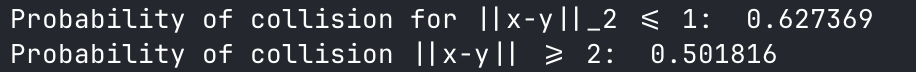
\includegraphics[scale=0.7]{ouput.png}
  \caption{Output of Python code}
\end{figure}

\section*{Problem 3}
Let $X \in \R^{d \times n}$ and define the kernel matrix as $K_{ij} = k(x_i,x_j)$ for kernel function $k$. We define the diagonal matrix $D$ as $D_{ii} = \sum_{j=1}^n K_{ij}$ and get the Laplacian of the graph as $L = D - K$. Then the normalized Laplacian is computed as 

\begin{equation*}
  D^{-1/2}LD^{-1/2} = I - D^{-1/2}KD^{-1/2} \implies D^{-1/2}KD^{-1/2} = I - D^{-1/2}LD^{-1/2}
\end{equation*}
then if $y = D^{1/2}x$, where $x$ is an eigenvector of $L$, then we have that
\begin{align*}
  D^{-1/2}LD^{-1/2}y &= D^{-1/2}LD^{-1/2}D^{1/2}x = D^{-1/2}Lx = D^{-1/2}(\lambda x) = \lambda y
\end{align*}
and
\begin{equation*}
  D^{-1/2}KD^{-1/2}y = (1-\lambda)y
\end{equation*}
thus the eigenvectors of $D^{-1/2}KD^{-1/2}$ are the same as the eigenvectors of $D^{-1/2}LD^{-1/2}$, but are reversed in order. Now since the row sum of $L$ is always zero, we have that the lowest eigenvalue is $0$ with corresponding eigenvector of all $1$'s and hence we take the first $2$ eigenvectors of $L$, corresponding to the two lowest singular vectors of $L$. We then use thses singular vectors to construct a projection matrix that maps into the space spanned by these two vectors, and then apply $k$-means to this projected data to form our clusters of $k=2$, thus we are choosing the second largest eigenvector of $D^{-1/2}KD^{-1/2}$.


\section*{Problem 4}
Let $X \subseteq \R^3$, and suppose that $k_1$ and $k_2$ are kernel functions on $X$, then we have that if $k(x,y) = k_1(x,y)k_2(x,y)$, then we have that
\begin{align*}
  k(x,y) &= k_1(x,y)k_2(x,y) = k_1(y,x)k_2(y,x) = k(y,x) \\
\end{align*}
and
\begin{align*}
  \sum_{i,j} k(x_i,x_j)c_ic_j = \sum_{i,j}k_1(x_i,x_j)k_2(x_i,x_j)c_ic_j = \sum_{i,j} k_1(x_i,x_j) \phi_2(x_i)c_i \phi_2(x_j)c_j = \sum_{i,j} k_1(x_i,x_j)d_i d_j \geq 0 
\end{align*}
Which is true since $k_1$ is a kernel function. Now if $k(x,y) = k_1(x,y) + k_2(x,y)$, then we have that
\begin{align*}
  k(x,y) &= k_1(x,y) + k_2(x,y) = k_1(y,x) + k_2(y,x) = k(y,x) \\
\end{align*}
and
\begin{align*}
  \sum_{i,j} k(x_i,x_j) c_ic_j  &= \sum_{k_1}(x_i,x_j)c_ic_j + \sum_{k_2}(x_i,x_j)c_ic_j \geq 0
\end{align*}
since $k_1$ and $k_2$ are kernel functions. Lastly, suppose that $k(x,y) = f(x)f(y)$, for $f: X \to \R$, then we have that
\begin{equation*}
  k(x,y) = f(x)f(y) = f(y)f(x) = k(y,x)
\end{equation*}
and
\begin{equation*}
  \sum_{i,j} k(x_i,x_j)c_ic_j = \sum_{i,j} f(x_i)f(x_j)c_ic_j = \left(\sum_{i} f(x_i)c_i\right)^2 \geq 0
\end{equation*}
thus $k$ is a kernel function.

\section*{Problem 5}
First recall for kernel $k$-means we have that
\begin{equation*}
  \norm{\phi(x_i) - \mu_C}_2^2 = k(x_i,x_i) + \frac{1}{n_C^2} \sum_{\ell,j \in C}k(x_\ell,x_j) - \frac{2}{n_C} \sum_{j \in C}k(x_i,x_j)
\end{equation*}
then for a given iteration and single data point $x_i$, we have that worst-case complexity is given by $O(dn^2)$, since if we consider the case where all points are allocated to a single cluster, then computing $k(\mu_C,\mu_C)$ would require $n^2$ computations of $k$ with complexity of $O(d)$. Then if we sum over all $x_i$ in our data set, we get that our overall complexity for a single iteration is $O(dn^3)$. For the case where $K$ is a Nystrom approximation of rank $k$, we have that the complexity of computing $K$ is $O(dnk)$, and hence the complexity of a single iteration is $O(dnk^2)$.

\end{document}
